\documentclass{jsarticle}
\usepackage{moreverb}
\usepackage[dvipdfmx]{graphicx}
\usepackage{float}

\title{計算機実習 問題6.8 - 他の1次元写像}
\author{早稲田大学先進理工学部物理学科 B4 藤本將太郎}
\date{2014/05/08}

\begin{document}
\maketitle

	\section{シミュレーションの目的}
		このシミュレーションの目的は、1次元写像
		\begin{equation}
			f(x)=xe^{r(1-x)}
			\label{eq:e1}
		\end{equation}
		
		\begin{equation}
			f(x)=r\sin{\pi x}
			\label{eq:e2}
		\end{equation}
	
		の定性的な性質を調べることである。写像(\ref{eq:e1})は、伝染病の影響で個体数に上限のある生態系モデルの研究のために、生態学者たちに用いられた。これは、問題6.1で考えた写像
		
		\begin{equation}
			f(x)=4rx(1-x)
			\label{eq:e3}
		\end{equation}
		
		よりもさらに複雑であるが、初期の個体数にどんな正の値を用いても、その個体数が正になることが好都合な点である。$r$の最大値には制限はないが、$r$が十分に大きくなると、$x$は実質的に0になり、その生物は絶滅してしまう。$0 < r \le 1 $および$0 \le x \le 1$とした正弦関数による写像(\ref{eq:e2})は、非線形である以外には特別なことはない。

	\section{作成したプログラム}
		本シミュレーションでは、問題6.1や6.2で行ったように、異なる初期値$x_{0}$に対して時系列の発展の様子はどうなるか、また、十分時間の経過した後の$x$の振る舞いは、$r$によってどのように変化するか、ということをシミュレーションする。したがって問題6.1と問題6.2のプログラムの時間発展方程式の部分を書き換えるだけでよく、これらをパッケージ化したものを利用して、実行プログラムの中では関数の定義とパラメータの代入のみを行うように改良した。以下に作成したプログラムを列挙する。
		
		\subsection{パラメータの設定ダイアログ(SetParameter.py)}
			\listinginput{1}{SetParameter.py}
		
		\subsection{与えられた関数とパラメータに関して時系列変化を描画するプログラム \\ (myplot\_6\_8\_iterate.py)}
			\listinginput{1}{myplot_6_8_iterate.py}
		
		\subsection{与えられた関数とパラメータに関してBifurcation Diagramを描画するプログラム(myplot\_6\_8\_bifurcation.py)}
			\listinginput{1}{myplot_6_8_bifurcation.py}
		
		\subsection{式(\ref{eq:e1})の時系列変化を描画するプログラム(6-8\_example1.py)}
			\listinginput{1}{6-8_example1.py}
		
		\subsection{式(\ref{eq:e1})のBifurcation Diagramを描画するプログラム(6-8\_example1\_bifurcation.py)}
			\listinginput{1}{6-8_example1_bifurcation.py}
		
		\subsection{式(\ref{eq:e2})の時系列変化を描画するプログラム(6-8\_example2.py)}
			\listinginput{1}{6-8_example2.py}

		\subsection{式(\ref{eq:e2})のBifurcation Diagramを描画するプログラム(6-8\_example2\_bifurcation.py)}
			\listinginput{1}{6-8_example2_bifurcation.py}

	
	\section{実習課題}
	
		\begin{enumerate}
			\renewcommand{\labelenumi}{\alph{enumi}.}
			\renewcommand{\labelenumii}{}
			
			\item $r=1.5, 2, 2.7$のとき、式(\ref{eq:e1})の時系列はどのような振る舞いを示すか。$f(x)$の定性的な振る舞いについて述べよ。極大点は存在するか。(補充課題)式(\ref{eq:e2})の定性的な振る舞いについても調べる。
			
			\begin{enumerate}
				\item まず、2.4のプログラムを用いて、$r=1.5, 2, 2.7$としたときの式(\ref{eq:e1})の時系列変化の様子を調べた。これらの実際のグラフを図\ref{fig:f1}、\ref{fig:f2}、\ref{fig:f3}に示した。それぞれのグラフはいくつかの初期条件$x_{0}$について調べてある。これらのグラフから分かることとして、$r=1.5$のときアトラクタは$x=1$であり、$x > 0$の任意の初期値に対して十分時間が経過すると周期1の運動となる。$r=2.0$の時には、系は$x=1$に周期2で振動しながら近づいていくことがわかる。$r=2.7$の時には周期8より大きい周期で振動しており、カオス的な振る舞いを見せることが分かる。
				\begin{figure}[H]
				\begin{center}
				\begin{tabular}{cc}
					\begin{minipage}{0.46\hsize}
						\begin{center}
							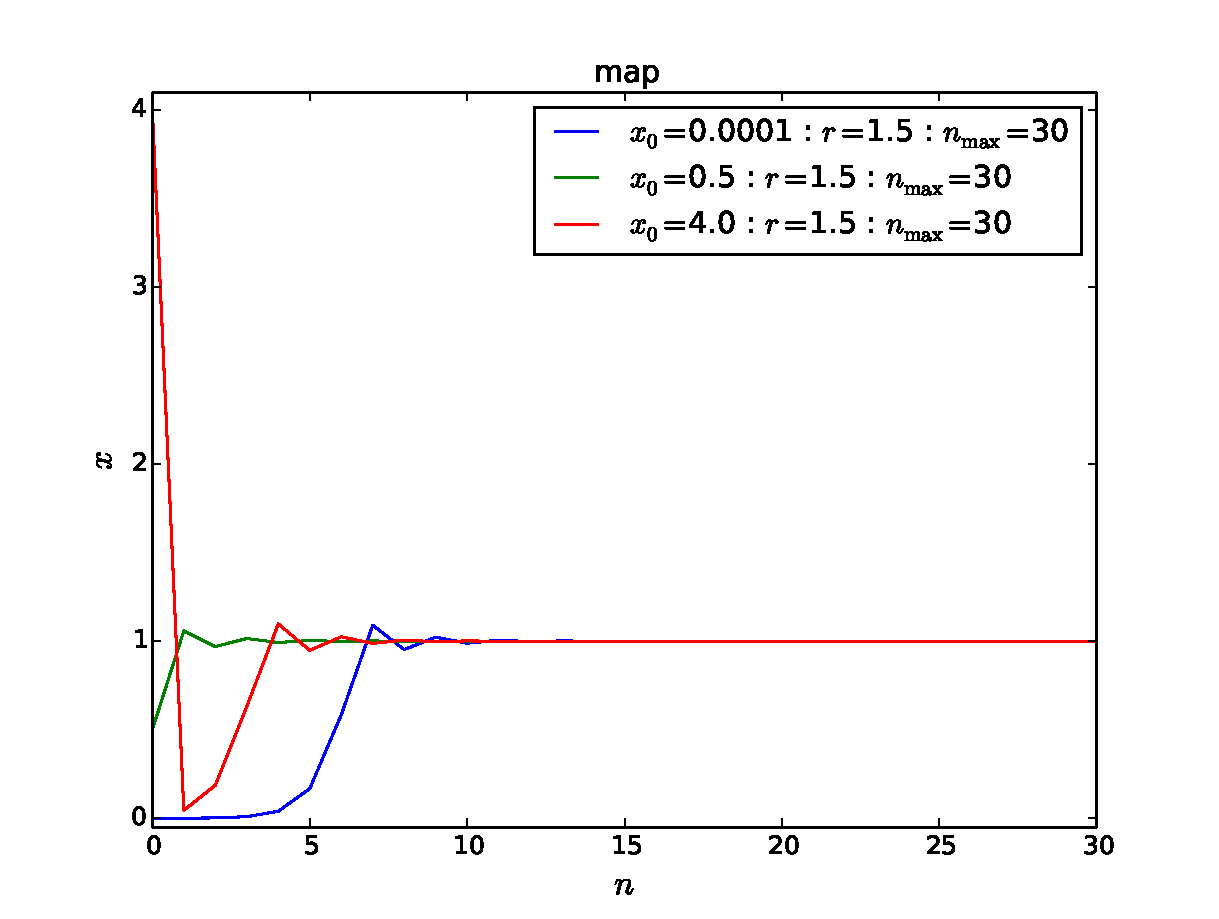
\includegraphics[width=7.3cm]{figure_1-1.pdf}
							\caption{$r=1.5$で$x_{0}=0.0001, 0.5, 4.0$とした時のグラフ}
							\label{fig:f1}
						\end{center}
					\end{minipage}
				
					\begin{minipage}{0.46\hsize}
						\begin{center}
							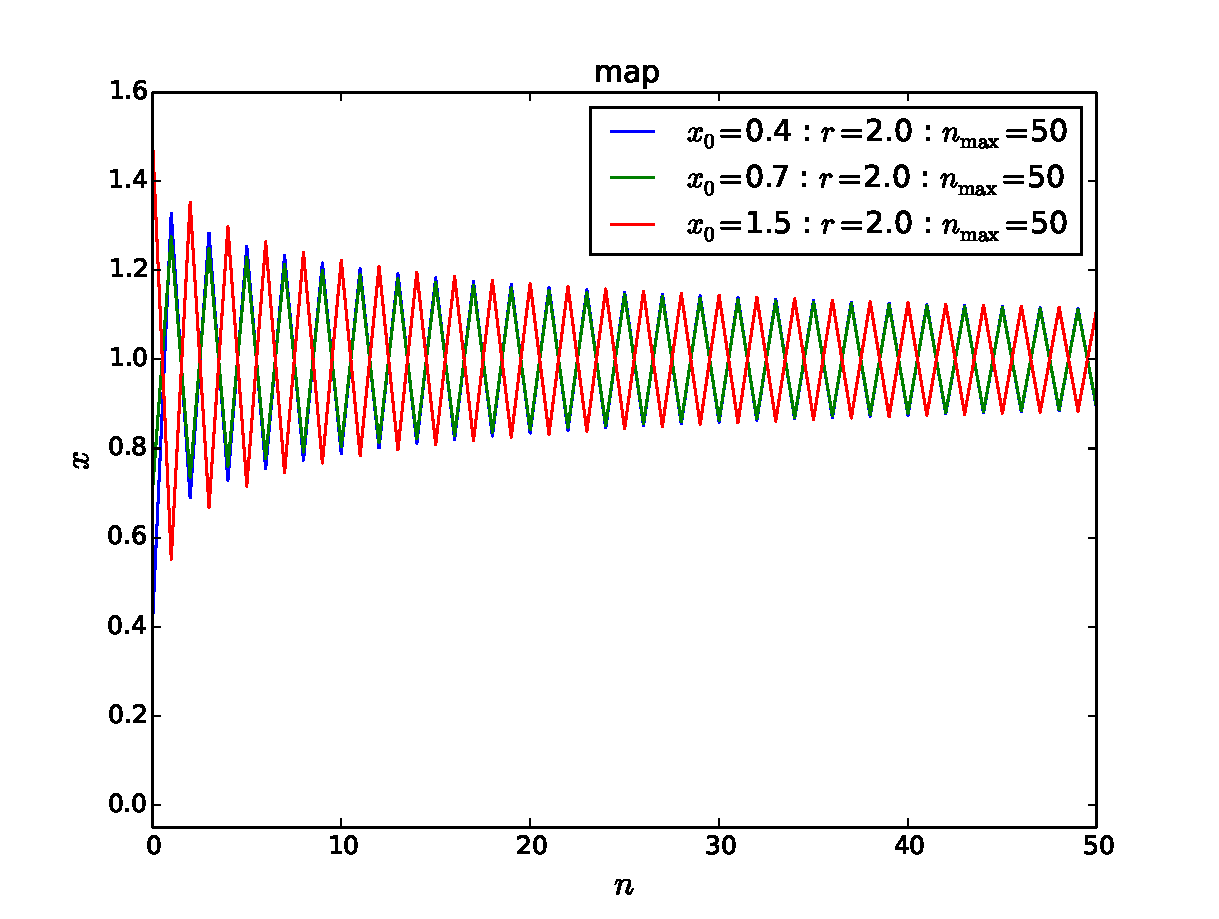
\includegraphics[width=7.3cm]{figure_1-2.pdf}
							\caption{$r=2.0$で$x_{0}=0.4, 0.7, 1.5$とした時のグラフ}
							\label{fig:f2}
						\end{center}
					\end{minipage}
					
					\\
					
					\begin{minipage}{0.46\hsize}
						\begin{center}
							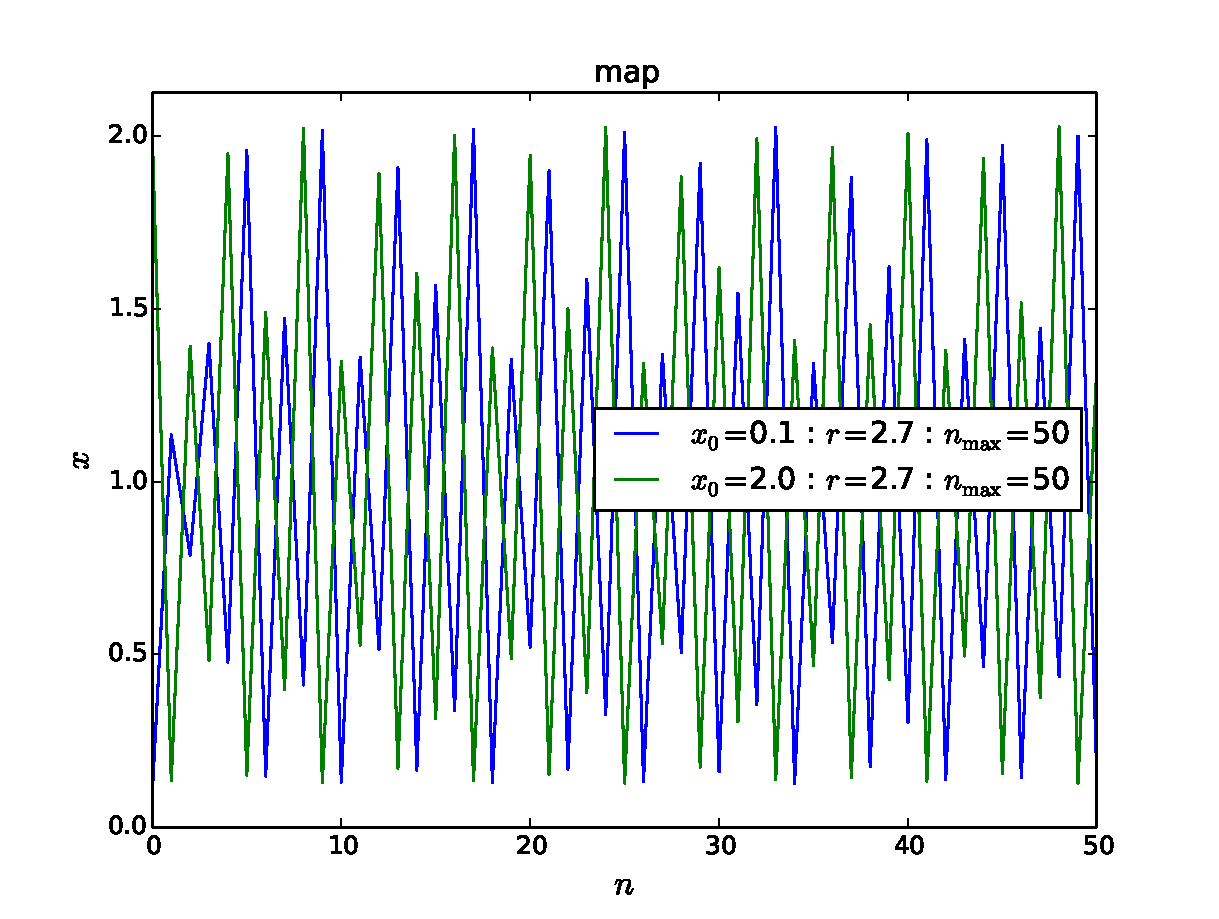
\includegraphics[width=7.3cm]{figure_1-3.pdf}
							\caption{$r=2.7$で$x_{0}=0.1, 2.0$とした時のグラフ}
							\label{fig:f3}
						\end{center}
					\end{minipage}
					
				\end{tabular}
				\end{center}
				\end{figure}
				
				次に、適当な初期値$x_{0}$のもとで、十分時間が経過した後の$x$の値を$r$に関してプロットし、$x$と制御パラメータ$r$の定性的な関係について考える。$x_{0}=0.5$、$r$の刻み幅$dr=0.001$として、はじめの1000回の計算結果は無視し、その後の50回を赤、さらにその後の50回を青でプロットしたものを図\ref{fig:f4}に示す。このグラフから、先ほど考慮した時間発展についてさらに多くの示唆が与えられる。例えば$r=2.0$のとき、図\ref{fig:f2}からだけでは、十分時間の経過した後に$x$は1に収束するのか、それとも周期2で振動するのかがわからないが、図\ref{fig:f4}を見ると、$r=2.0$の付近で周期1から周期2への周期倍化が起こっていることが見て取れる。分岐点の位置を詳細に知るために、$r=2.0$の部分を拡大し、さらに演算回数を増やしてみると(ntransient=1000000)、ちょうど$r=2.0$で分岐することが分かる(図\ref{fig:f4-2})。
				
				\begin{figure}[H]
					\begin{center}
						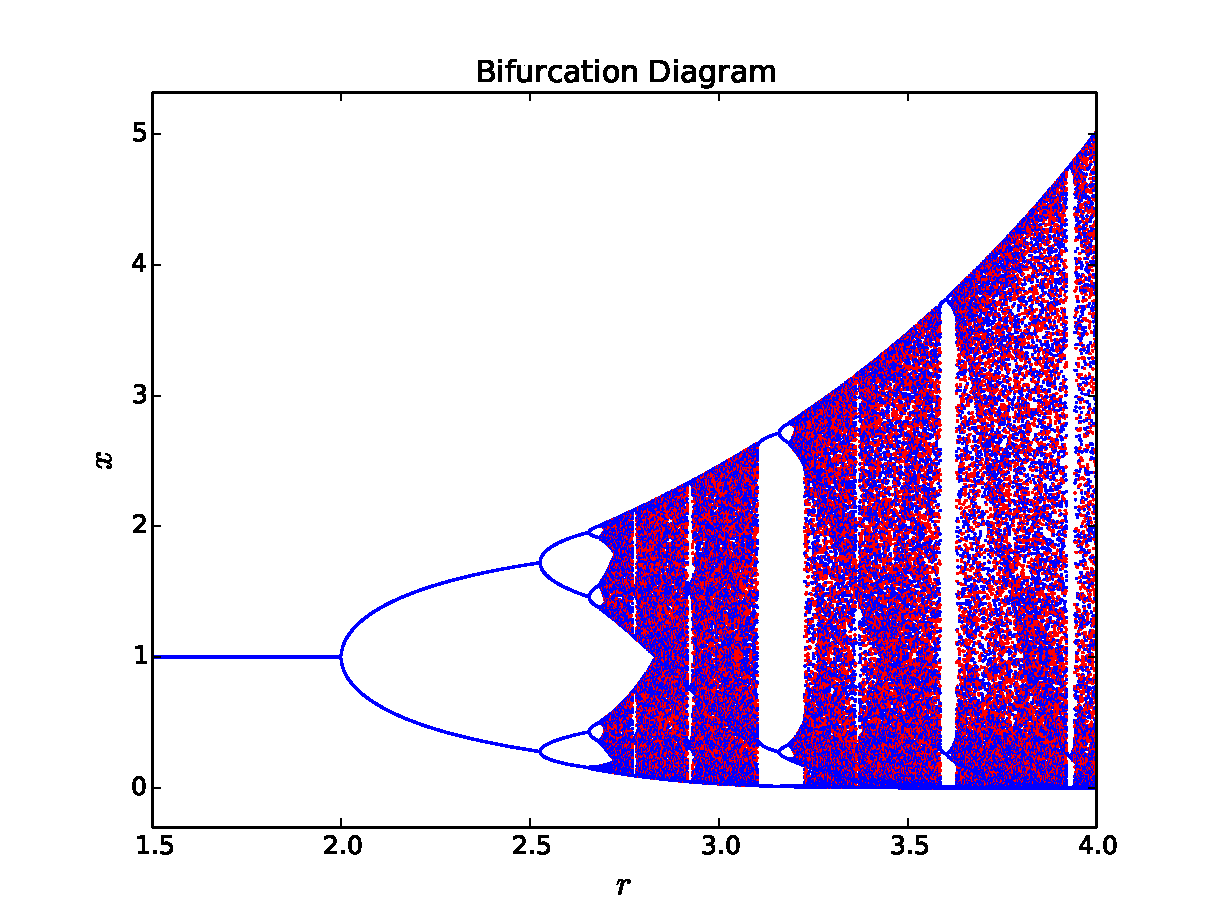
\includegraphics[width=12.5cm]{figure_1-4.pdf}
						\caption{式(\ref{eq:e1})におけるパラメータ$r$と$x$の関係}
						\label{fig:f4}
					\end{center}
				\end{figure}
				
				\begin{figure}[H]
					\begin{center}
						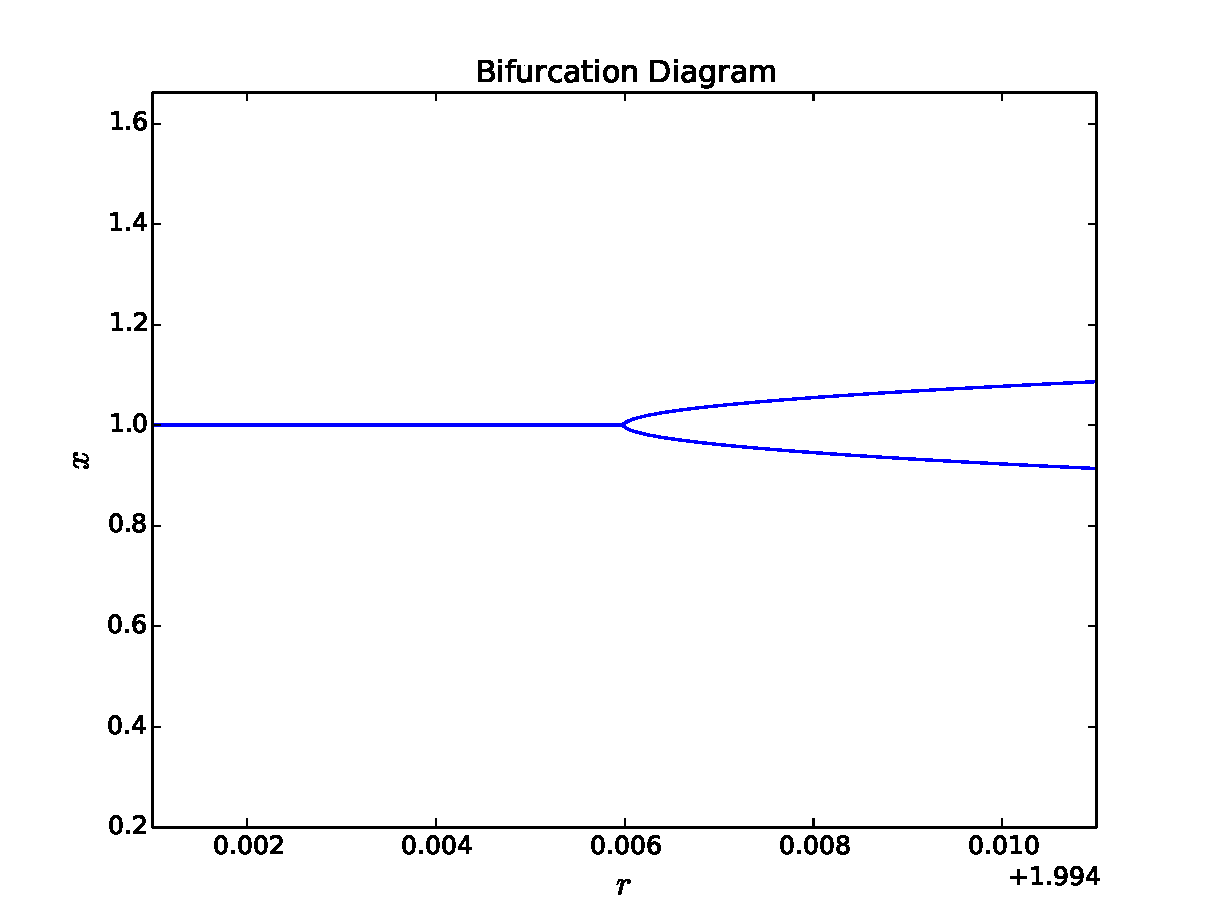
\includegraphics[width=12.5cm]{figure_1-4-2.pdf}
						\caption{$r=2.0$の近傍での$x$の振る舞い($\mathrm{dr}=0.00001$)}
						\label{fig:f4-2}
					\end{center}
				\end{figure}
				
				\item 式(\ref{eq:e2})のBifurcation Diagramを図\ref{fig:f5}に示す。ここで初期値$x_{0}=0.5$、プロットしない演算回数$\mathrm{ntransient}=1000$、プロットする回数$\mathrm{nplot}=50$、$r$の刻み幅$\mathrm{dr}=0.001$とした。このグラフから、$r=0.32$付近で挙動が変化し($1<x_{0} \le 2$のときはちょうど$x=0$で折り返した形)、$r=0.71$で周期が2に変化している。次に$r=0.83$のあたりでさらに周期が4に変化し、$r=0.86$で周期8となって、その後すぐ周期16となっている。このように周期倍化の様子が観察され、以降の挙動はカオス的であることもわかる。$r=0.94$付近での周期3となる窓など、いくつかの窓があることも観察される。
				\begin{figure}[H]
					\begin{center}
						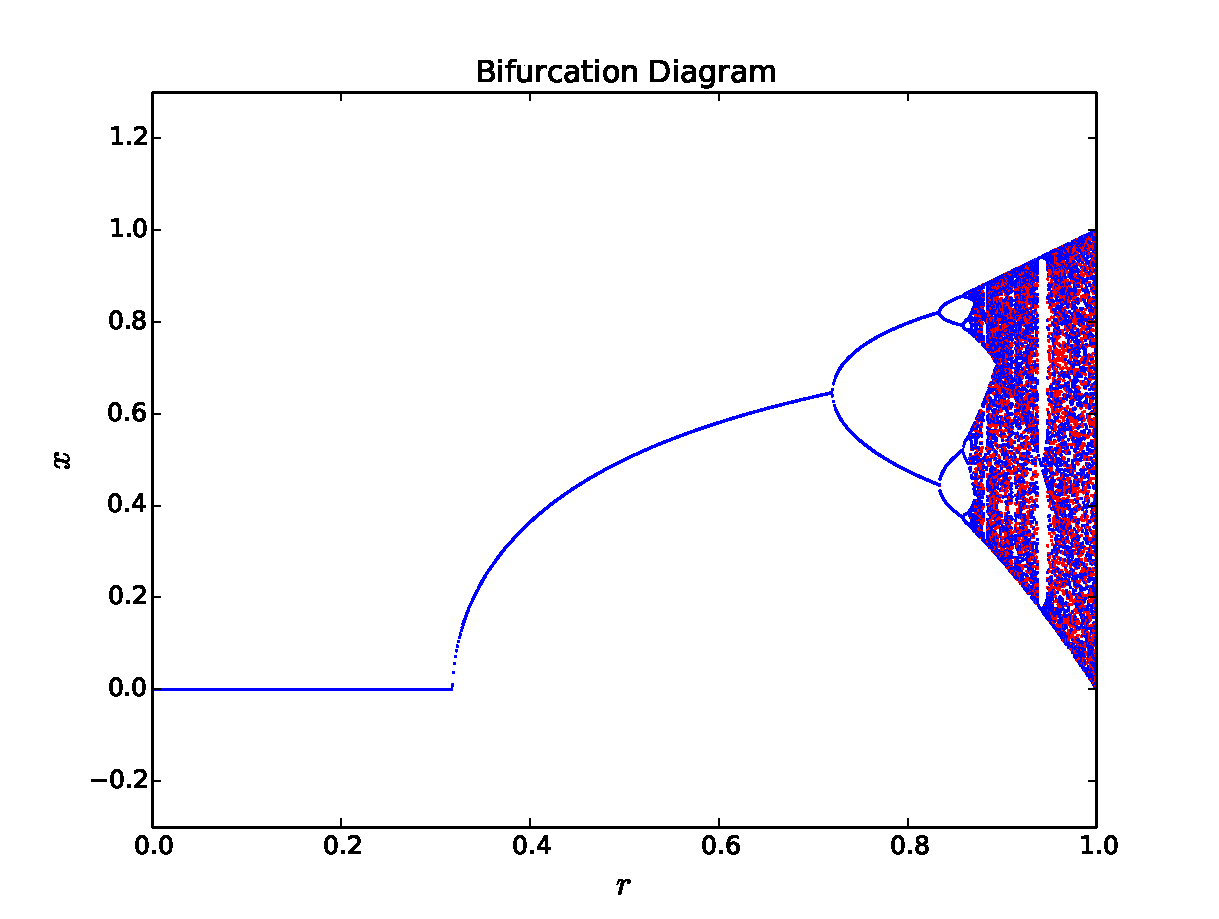
\includegraphics[width=12.5cm]{figure_2-1.pdf}
						\caption{$r$に対する過渡現象以後の$x$の振る舞い}
						\label{fig:f5}
					\end{center}
				\end{figure}
			
			\end{enumerate}
			
		\end{enumerate}
	
	\section{まとめ}
		1次元写像(\ref{eq:e1})、(\ref{eq:e2})の定性的な振る舞いについて調べることを通して、ロジスティック写像以外の1次元写像におけるカオス的挙動と、そこに至るまでの周期倍化などについて理解を得ることができた。分岐点の位置$r$から$\delta$を算出する問題については、今後取り組むことにしたい。
	
	\section{参考文献}
		\begin{itemize}
			\item ハーベイ・ゴールド,ジャン・トボチニク,石川正勝・宮島佐介訳『計算物理学入門』,ピアソン・エデュケーション, 2000.
		\end{itemize}

\end{document}
